\section{Senior/Key Personnel Profile}
\subsection{Carl Brandon}
\subsubsection{Significant Publications}
\begin{itemize}
\item From Physicist to Rocket Scientist and How to Make a CubeSat
  That Works \cite{brandon:2020}
\end{itemize}

\subsubsection{Commitment}
\begin{description}
\item[Research] 1,500 hours per year
\item[Lectures]   450 hours per year
\item[Grad Students] 0
\end{description}

\subsubsection{Other Support}
At the present there is no other financial support available.

\subsection{Peter Chapin}
%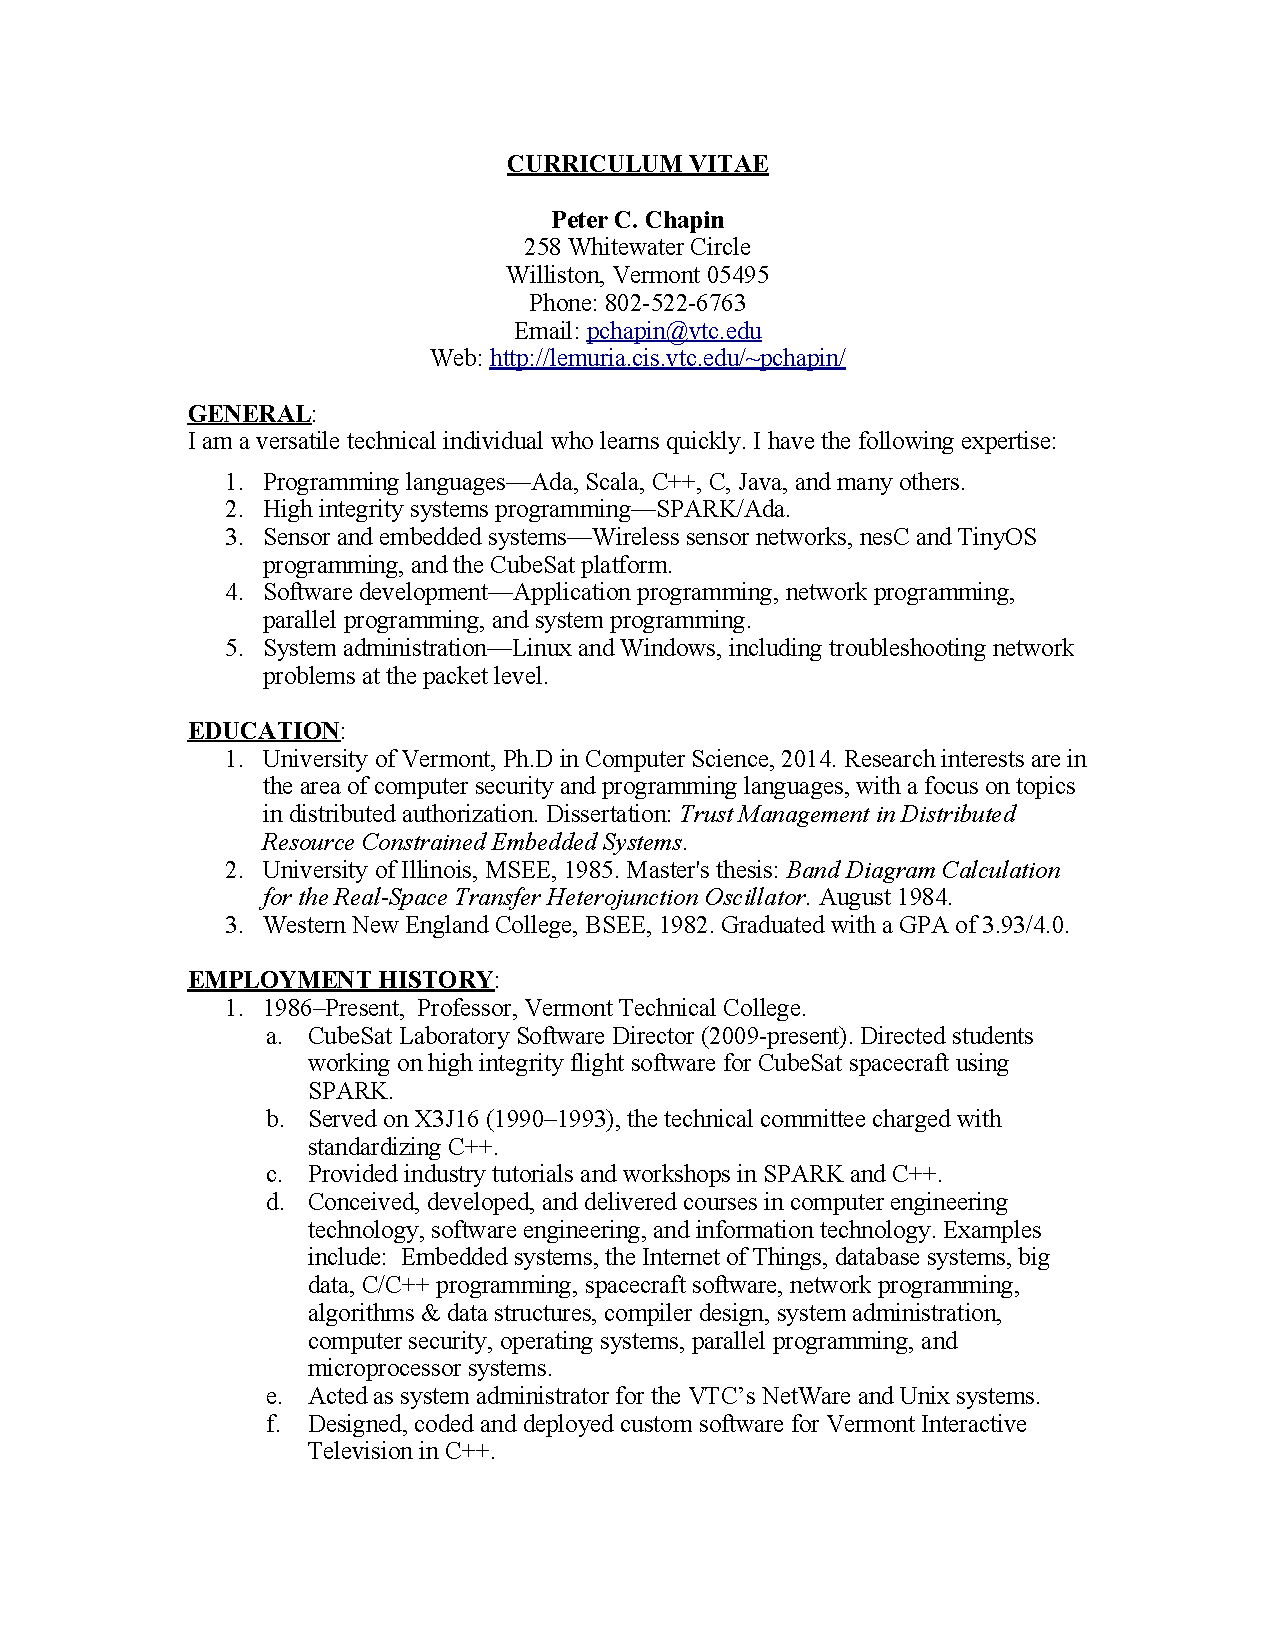
\includepdf[pages={-}]{./pdf/peter-chapin-cv.pdf}
\subsubsection{Significant Publications}
\begin{itemize}
\item Building High Integrity Applications with SPARK\cite{chapin:2015}
\end{itemize}

\subsubsection{Commitment}
\begin{description}
\item[Research] 1,500 hours per year
\item[Lectures]   450 hours per year
\item[Grad Students] 2
\end{description}

\subsubsection{Other Support}
At the present there is no other financial support available.

\subsection{Hamid Ossareh}
%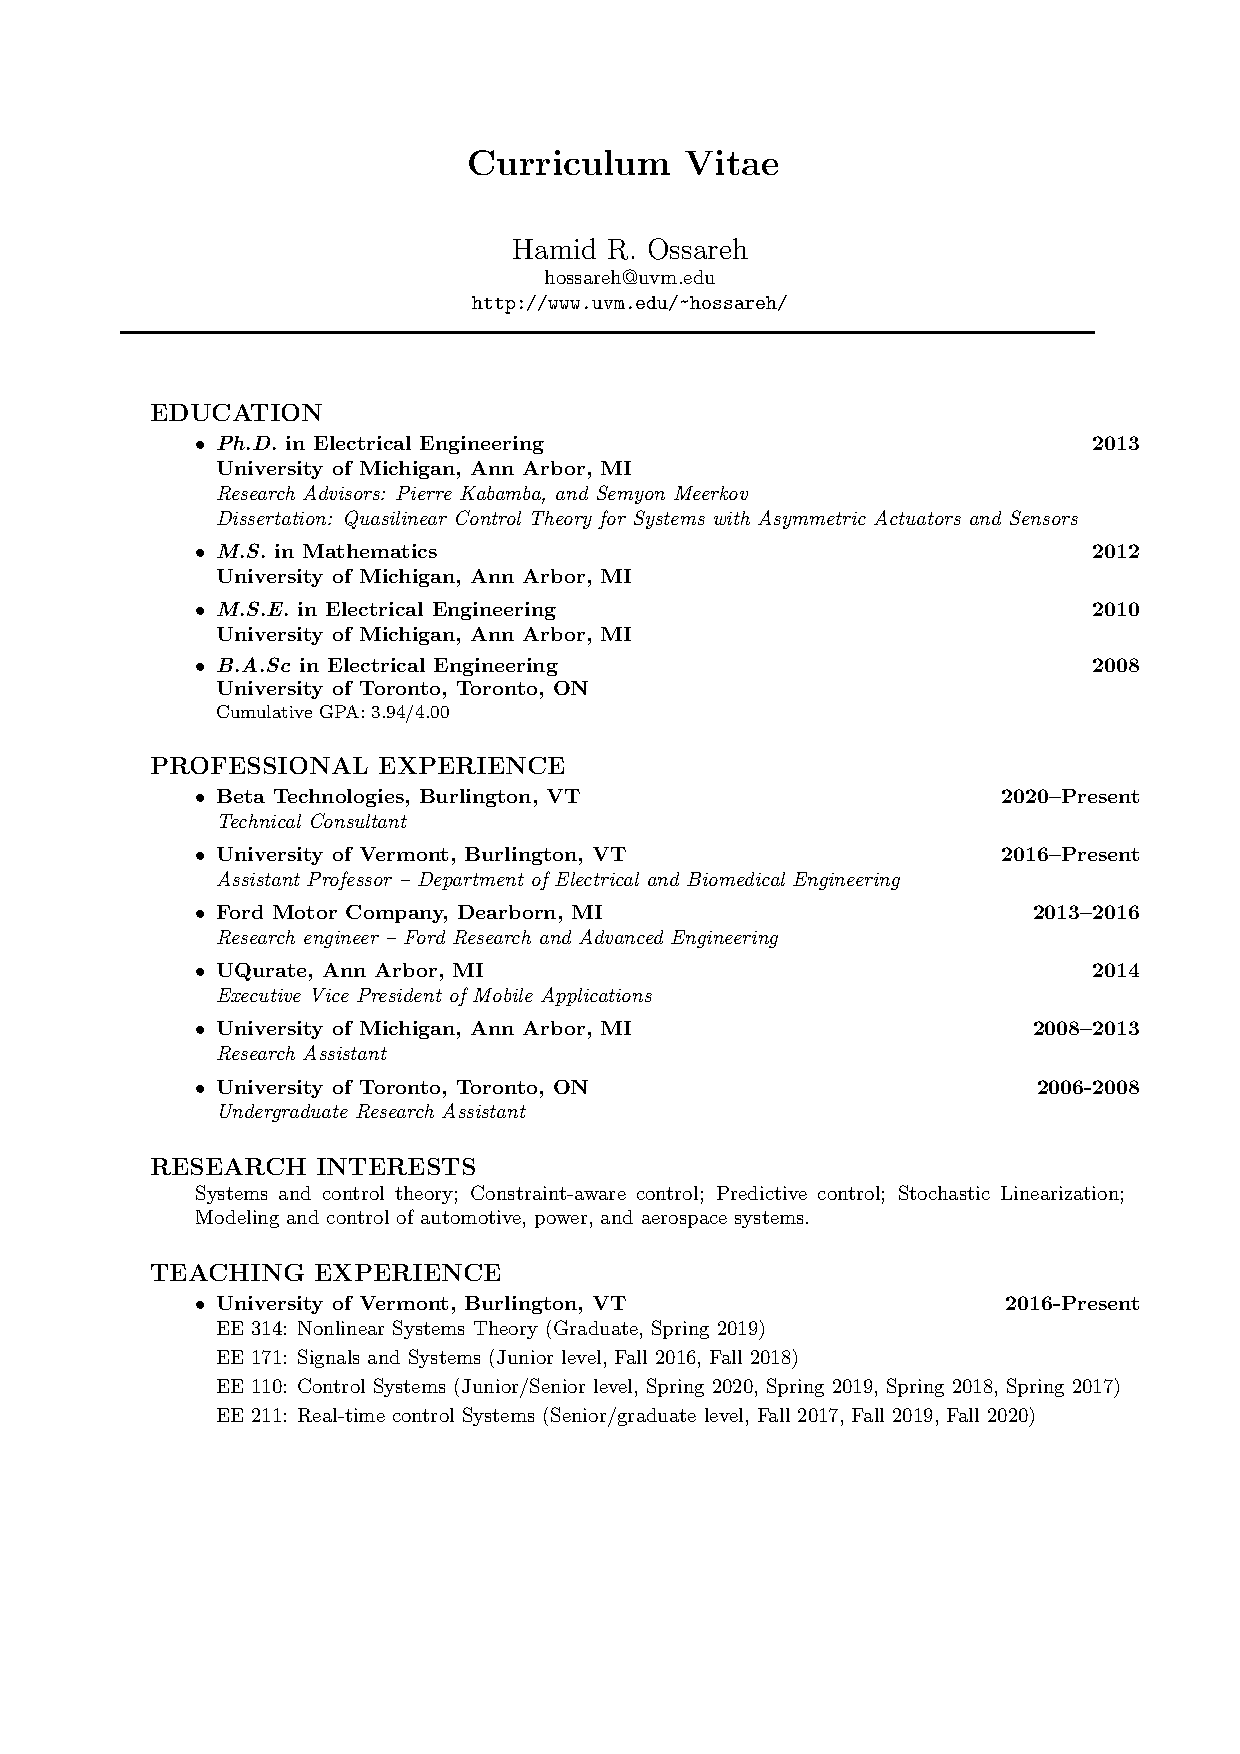
\includepdf[pages={-}]{./pdf/hamid-ossareh-cv.pdf}
\subsubsection{Significant Publications}

\begin{itemize}
\item S. Brahma, M. R. Almassalkhi, H. R. Ossareh. ``Optimal Control
  of Virtual Batteries using Stochastic Linearization'', IEEE
  Conference on Control Technology and Applications (CCTA). 2021.
\item S. Brahma, T. Foley, S. Wisotzki, H. R. Ossareh, ``An
  Investigation into Accuracy, Computation, and Robustness of
  Stochastic Linearization of Systems with Saturation
  Nonlinearities''. Results in Control and Optimization. 2021.
\item S. Brahma, N. Nazir, H. R. Ossareh, and M. Almassalkhi,
  ``Optimal and resilient coordination of virtual batteries in
  distribution feeders''. IEEE Transactions on Power Systems. 2020.
\item P. Kabamba, S. Meerkov, H. R. Ossareh. ``Stochastic
  Linearisation Approach to Performance Analysis of Feedback Systems
  with Asymmetric Nonlinear Actuators and Sensors''. International
  Journal of Control. 2014.
\item S. Brahma, H. R. Ossareh. ``Quasilinear Control of Feedback
  Systems with Multivariate Nonlinearities''. Proceedings of the 2019
  IEEE Conference on Decision and Control (CDC). 2019.
\end{itemize}

\subsubsection{Commitment}
\begin{description}
\item[Research] 100 hours per year
\item[Other Research] 1,000 hours per year
\item[Lectures]  450 hours per year
\item[Grad Students] 1
\end{description}

\subsubsection{Other Support}
At the present there is no other financial support available.

